\documentclass[twocolumn,10pt]{asme2ej}

\usepackage{epsfig} 

\title{%
	Personenzentrisches Projektmanagement\\
	\large 
	- \\
	Einfluss verschiedener Persönlichkeiten auf \\ 
	das Projektmanagement von Data Science Projekten}

\author{Tobias Rohrer
    \affiliation{
	Hochschule Darmstadt\\
	Data Science (Master)\\
    Email: sttorohr@stud.h-da.de
    }	
}

\graphicspath{ {./images/} }
\usepackage[center]{caption}
\usepackage[locale=DE]{siunitx}
\usepackage{hyperref}

\usepackage{listings}
\usepackage{xcolor}
\usepackage{enumitem}
\definecolor{codegreen}{rgb}{0,0.6,0}
\definecolor{codegray}{rgb}{0.5,0.5,0.5}
\definecolor{codepurple}{rgb}{0.58,0,0.82}
\definecolor{backcolour}{rgb}{0.95,0.95,0.92}

\lstdefinestyle{mystyle}{
	backgroundcolor=\color{backcolour},   
	commentstyle=\color{codegreen},
	keywordstyle=\color{magenta},
	numberstyle=\tiny\color{codegray},
	stringstyle=\color{codepurple},
	basicstyle=\ttfamily\footnotesize,
	breakatwhitespace=false,         
	breaklines=true,                 
	captionpos=b,                    
	keepspaces=true,                 
	numbers=left,                    
	numbersep=5pt,                  
	showspaces=false,                
	showstringspaces=false,
	showtabs=false,                  
	tabsize=2
}
\lstset{style=mystyle}
\begin{document}

\maketitle    

%%%%%%%%%%%%%%%%%%%%%%%%%%%%%%%%%%%%%%%%%%%%%%%%%%%%%%%%%%%%%%%%%%%%%%
\begin{abstract}


\end{abstract}

%%%%%%%%%%%%%%%%%%%%%%%%%%%%%%%%%%%%%%%%%%%%%%%%%%%%%%%%%%%%%%%%%%%%%%
\section{Einleitung}
Methoden und Werkzeuge zum Managen von Projekten werden meist anhand des Projektumfangs, Komplexität oder der Klarheit von Anforderungen ausgewählt. Außer acht gelassen wird dabei jedoch, dass sich ein Projektteam aus verschiedenen Persönlichkeiten mit unterschiedlichen Stärken und Schwächen zusammen setzt. Einer der Punkte im Agilen Manifesto lautet sogar "Individuals and interactions over processes and tools" \cite{beck2001agile}. Im Folgenden wird Diskutiert, wie sich verschiedene Projektmanagement-Werkzeuge und Methoden auf die Stärken und Schwächen, sowie auf die Motivation der Persönlichkeiten nach dem DISC-Modell auswirken.

Dazu wird in Abschnitt \ref{sec:1} zunächst das Projektmanagement in Data Science Projekten via Scrum, Kanban und dem Wasserfallmodell, sowie die darin verwendeten Projektmanagement-Werkzeuge gegenüber gestellt.

In Abschnitt \ref{sec:2} werden anschließend die einzelnen Persönlichkeitskategorien nach dem DISC-Modell beschrieben. Außerdem wird diskutiert, wie die Projektmanagement-Methoden und Werkzeuge aus Abschnitt \ref{sec:1} unter Berücksichtigung der Stärken und Schwächen der am Team teilnehmenden Persönlichkeiten eingesetzt werden sollten.


\section{Projektmanagement in Data Science Projekten}\label{sec:1}
Es gibt unzählige Methoden, um Projekte zu verwalten. Im Folgenden werden 3 der meist verbreitetsten kurz beschrieben\footnote{Ausführlichere Beschreibungen der Methoden in den Quellen.}. Anschließend werden die Besonderheiten von Data Science Projekten erläutert und die drei zuvor beschriebenen Methoden im Bezug auf diese Besonderheiten gegenüber gestellt.

\subsection{Wasserfallmodell}
Das Wasserfallmodell lässt sich am besten durch seine sequenziell ablaufenden Phasen charakterisieren. Eine neue Phase wird erst nach erfolgreichem Abschluss der vorgeschalteten Phase gestartet. Zwar bietet das Wasserfallmodell eine gute Übersicht über die Gesamtplanung des Projekts, doch ist es relativ unflexibel gegenüber Veränderungen. \cite{Wasserfall}

\subsection{Agile}
Scrum und Kanan gehören beide zur Gruppe der Agilen Methoden und teilen demnach deren Grundprinzipien. Diese sind im Agile Manifesto gestgehalgen und sind:
- Shortest Path. Reduce Wait times...
\cite{beck2001agile}


\subparagraph{Scrum}
Die Grundiee von Scrum ist die Einteilung des Projektes in Inkremente. Jedes Inkrement wird innerhalb eines sogenannten Sprints bearbeitet und anschließend ausgeliefert. Somit kann kontinuierlich Rückmeldung des Kunden in den Entwicklungsprozess einfließen. In einem Team, das nach Scrum arbeitet gibt es feste Rollen wie den Product Owner, den Scrum Master sowie das Projekt Team. Dem Product Owner obliegt üblicherweise die inhaltliche und dem Scrum Master die organisatorische Verantwortung.

\subparagraph{Kanban}
Angefangene Aufgaben schnellst möglich fertig zu stellen ist eines der zentralen Punkte von Kanban. Um dies zu unterstützten wird üblicherweise ein work in progress (WiP) limit definiert, um sich auf angefangene Aufgaben zu konzentrieren und deren Fertigstellung zu beschleunigen. Dieser Prozess wird auf einem gemeinsamen Kanban Board visualisiert. Hierauf werden die aktuellen Aufgaben, sowie deren Status dargestellt. Ein weiteres Ziel die kontinuierliche Effizienzsteigerung dieses Prozesses.\cite{kanban} Aktualisierungen werden an den Kunden ausgeliefert, sobald Sie fertig sind. In Kanban gibt es keine festen Teamrollen. Üblicherweise wird der Kanban Prozess durch die sogenannte Lead und Cycle Zeit überwacht. Diese misst die Zeit, die eine Aufgabe von der Aufnahme bis zur fertigstellung benötigt. Der Prozess, mit dem das Projektmanagement nach Kanban aufgebaut wird kann sich jederzeit ändern. Im Vergleich zu Scrum kann man Kanban als eher kontinuierliche Methode sehen, wobei Scrum auf feste Inkremente mit definiertem Start und Ende (Sprints) arbeitet.

\subsection{Besonderheiten von Data Science Projekten}
Bei Data Science Projekten ist zu Projektstart oft nicht genau abzuschätzen, ob und in wie fern die festgelegten Ziele mit den verfügbaren Daten erreicht werden können. Dies liegt unter anderem daran, dass die Qualität der zu verarbeitenden Daten fehl eingeschätzt wird. Diese wird in der Praxis eher über statt unterschätzt. Unter Anderem findet deshalb die Auswahl der einzusetzenden Technologien oft erst im laufe des Projektes statt \cite{agile_pm}. Darüber Hinaus können sich die Anforderungen im Laufe des Projektes ändern. Beispielsweise werden durch die Verarbeitung der Daten neue Möglichkeiten vom Entwicklungsteam aber auch von den "Kunden" überhaupt erst erkannt. 

\subsection{Die Auswahl einer passenden Methode}

\begin{figure}
	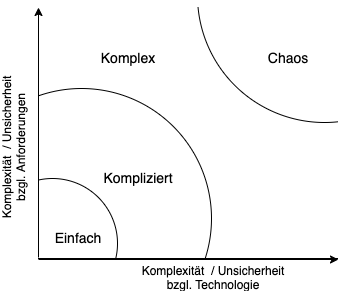
\includegraphics[scale=0.65	]{stacey.png}
	\caption[center]{Die Stacey Matrix angelehnt an \cite{stacey_img}}
	\label{fig:stacey}
\end{figure}

Eine Herausforderung zu beginn vieler Projekte stellt die Wahl einer passenden Projektmanagement Strategie da. Hierbei kann die Stacey Matrix \cite{Stacey2011StrategicMA} unterstützen, indem Projekte in Einfach, Kompliziert, Komplex oder Chaotisch klassifiziert werden (siehe Abbildung \ref{fig:stacey}). Die Klassifizierung wird anhand der Unklarheit und Komplexität der eingesetzten Technologien (Wie wird das Projekt umgesetzt), sowie der Klarheit über die Anforderungen an das Projekt (Was wird in dem Projekt umgesetzt) vorgenommen. Bei einer Klassifizierung im "oberen" komplizierten Bereich bis hin zum Chaotischen Bereich sollten Methoden aus dem Agilen Umfeld, in unserem Fall Kanban oder Scrum eingesetzt werden. Bei einer Klassifizierung als Einfach oder im unteren Komplizierten Bereich kann, muss aber nicht, auch das Wasserfallmodell verwendet werden. Durch die oben beschriebenen Unklarheiten bezüglich der Technologien sowie der Ziele sind die meisten Data Science Projekte in der Stacey Matrix eher ab der komplizierten Stufe einzuordnen. Das Wasserfallmodell ist für die meisten Data Science Projekte wegen der Inflexibilität gegenüber unvorhersehbaren kurzfristigen Abweichungen und Änderungen  eher ungeeignet.

\section{Einfluss von Persönlichkeiten auf das Projektmanagement}\label{sec:2}
Diese zuvor beschriebene Auswahl lässt aber die an dem Projektteam mitwirkenden Persönlichkeiten und deren stärken und schwächen außer acht. Im Folgenden werden zunächst verschiedene Persönlichkeitseigenschaften nach dem DISG-Modell erläutert. Anschließend werden deren typischen Stärken und Schwächen in Verbindung mit den Verschiedenen Projektmanagement Strategien diskutiert.

\subsection{Persönlichkeiten nach DISG}
Nach dem DISG-Modell \cite{disc} lassen sich Persönlichkeiten in die Bereiche Dominant(D), Initiativ(I), Stetig(S) und Gewissenhaft(G) unterteilen. Eine Persönlichkeit setzt sich meist aus unterschiedlichen Bereichen verschieden stark ausgeprägt zusammen. Mit Hilfe eines DISG-Persönlichkeitstests kann ein Persönlichkeitsprofil erstellt werden. Typische Eigenschaften der verschiedenen Persönlichkeitstypen können der folgenden Auflistung entnommen werden.

\begin{description}[align=left]
	\item [Dominant] Entschlossen, willensstark, direkt, herausfordernd, ergebnisorientiert, selbstbewusst, durchsetzungsfähig, risikobereit, sachlich
	\item [Initiativ] Optimistisch, kommunikativ, beeinflussend, enthusiastisch, emotional, anregend, spontan, gesellig, freundlich, unterhaltsam
	\item [Stetig] Loyal, hilfsbereit, geduldig, teamfähig, unterstützend, bescheiden, verbindlich, entspannt, zuverlässig, ausdauernd
	\item [Gewissenhaft] Hohe Maßstäbe, perfektionistisch, selbsdiszipliniert, vorsichtig, analytisch, zurückhaltend
	 \cite{disg_charakteristika}
\end{description}

%Ideen: Sind Dominant und Initiativ ungeduldig?
%

\subsection{Auswirkung verschiedene Projektmanagement Methoden auf die DISG Persönlichkeiten}
Auss den oben beschriebenen Charaktereigenschaften der verschiedenen Persönlichkeitstypen nach dem DISG-Modell ergeben sich unterschiedliche stärken und schwächen. Im Folgenden werden typische Stärken und Schwächen der Charaktere beschrieben und dargelegt, wie verschiedene Projektmanagement Methoden oder Werkzeuge verwendet werden können, um den Schwächen entgegenzuwirken und die Stärken zu nutzen.

Ziel ist ein motiviertes Team in dem jede Person ihre Stärken und Schwächen einbringen kann.

\subsection{Der Dominante}
\subparagraph{Motivation}
Der Dominante  wird vor Allem durch Erfolge und Herausforderungen motiviert. Unterstützt würde das beispielsweise durch eine Organisation nach Kanban. Durch das gesetzte WiP Limit und die daraus Verbunde Fokusierung auf wenige Aufgaben verringern sich die Zeiten bis zum Abschluss von einzelnen Aufgaben. Dadurch werden viele Erfolgserlebnisse erreicht, die sich motivierend auf die Dominante Persönlichkeit auswirken. Das Konzept, nach Kanban den Projektmanagement Prozess kontinuierlich zu verbessern kann außerdem als Herausforderung angesehen werden und sich motivierend auswirken.

Gerne hat er bei der Bewältigung von Aufgaben den Freiraum um Risiken einzugehen und um Entscheidungen zu treffen oder zumindest auf diese einzuwirken. In einer Organisation nach einer Agilen Methode ist das von Vorteil. In Wasserfall Bla.

Demotivierend würden sich beispielsweise monotone Routine artige Arbeitsbedingungen auswirken.

\subparagraph{Stärken und Schwächen}

Zu den größten Stärken des Dominanten gehört durch seine sachliche Art das Organisieren. Eine Organisation nach Kanban würde dem Dominanten den Raum geben, um Verbesserungen in der Organisation laufend einzubringen. 

Einer der größten Stärken des Dominanten ist seine Zielorientierte Arbeitsweise. 
Zielorientiert und einfallsreich Get things done !

Zu den Schwächen gehört, dass durch den Organisations und Diskussionsdrang zu viele Details zu ausgiebig diskutiert werden. Somit ist vor allem wichtig, dass in Daily Standup Meetings die ausgemachten Redezeiten eingehalten werden. 

Eine weitere Schwäche des Dominanten ist, dass er gerne Autoritäten überschreitet. Daher ist es zu empfehlen, bei einem Modell nach Kanban einer dominanten Persönlichkeit nicht die Aufgabe für die Kommunikation mit den Stakeholdern zu überlassen.

Des weiteren nimmt sich der Dominante gerne zu viel vor. Ein festes WiP Limit würde hier entgegen wirken. Ein Wasserfallmodell, in dem von vorne Herein ein Projektplan erstellt wird wäre hier Kontraproduktiv und würde wahrscheinlich zu Fehleinschätzungen kommen. Bei Scrum durch Sprint Planning und Story Points an denen die Teammitglieder mitschätzen. Hierbei ist zu beachten, dass bei der Abschätzung der Story Points der Dominante nicht zu viel Einfluss auf die Schätzungen anderer einnimmt (Planning Poker).

Der Dominante kann auch gerne unsensitiv gegenüber anderen sein. Es ist daher empfehlenswert öfter Retrospektiven durchzuführen um die Wogen zu Glätten. Hierbei sollte einer Dominanten Persönlichkeit zur Steigerung der Akzeptanz die die Vorteile einer Retrospektive zum erreichen der Projektziele klar gemacht werden.

\subparagraph{Fazit}

Heruntergebrochen auf die 3 Projektmanagement Methoden würde sich der Dominante wohl in einem Projekt, dass nach Kanban organisiert wird, am wohlsten und in einem Wasserfall-Projekt am unwohlsten fühlen.

\subsection{Die Initiative}
\subparagraph{Motivation}

Die Initiative fühlt in einer Umgebung, in der Sie ihre Ideen einbringen und andere davon überzeugen kann wohl. Gerne erfährt Sie Bestätigung in ihren Ideen durch die Unterstützung und positivem Feedback Anderer. Die Motivation der Initiativen hängt außerdem von ihrer wahrgenommenen Popularität im Team ab. Durch Lob, Unterstützung und Bestätigung kann somit die Motivation gesteigert werden. Generell wirkt sich ein freundliches und angenehmes Arbeitsklima positiv auf die Motivation aus.  Merge Requests mit Lob und nicht nur kühler Techy Kritik. 

\subparagraph{Stärken und Schwächen}
Durch ihre Überzeugungskraft und Optimismus kann Sie motivierend auf andere wirken. 
Kreativität. 
Da die Initiative oft Popularität in der Gruppe hat ist Sie eine gute Schlichterin in einer Gruppe.

Durch ihre kreativität und impulsivität ist Sie eine gute Ideengeberin. Dies kann sich jedoch auch als Schwäche herausstellen. Bei einem zu großen Hang zur Implusivität können gerne Details bei der Planung oder Durchführung von Aufgaben übersehen werden. Dies kann daran liegen, dass die Initiative schnell die Motivation an einer angefangenen Aufgabe verlieren kann. Je nachdem, wie Stark das Verhältnis von Kreativität und Impulsivität ausgeprät ist, könnte sich Scrum oder Kanban anbieten. Bei einer Organisation nach Scrum könnte man dem Impulsiven Drang durch den momentan festgelegten Sprint entgegenwirken. Das würde sich evtl. etwas demotivierend für die Initiative anfühlen, würde Sie aber dazu bringen aktuellen Arbeiten zunächst in entsprechender Qualität abzuschließen, bevor neue angefangen werden können. Bei einer Organisation nach Kanban könnte die Initiative aber besser ihre spontanen kreativen Einfälle einbringen.

Zu den Schwächen: 
Gibt nicht gerne negatives Feedback. Ignoriert Konflikte so lange wie möglich. 


\subsection{Der Stetige}
\subparagraph{Motivation}

Der Stetige wird unter Anderem durch die unterstützende Teilnahme an Aufgaben motiviert, ohne dabei aber als treibende Kraft mitzuwirken. Teammitgliedern zu helfen und dadurch Beziehungen aufzubauen bringt hierbei die Motivation. Eine Anerkennung dieser unterstützenden Art durch das Team wirkt sich hierbei besonders motivierend. Pair Programming? Code Review?	
 

Motiviert durch  Sicherheit?? (Eher Wasserfall, weil ein Plan? Oder auch Scrum, da Sprints?)
Aktivitäten die abgeschlossen werden können? 

\subparagraph{Stärken und Schwächen}

Stetige sind oft durch ihre empatischen und freundlichen Eigenschaften, sowie der Fähigkeit sich unterzuordnen bestens dafür Geeignet, um die Kommunikation mit Stakeholdern zu übernehmen. In einer Projektorganisation mit festen Rollen könnte diese Stärke unter gehen.

Nimmt sich gerne Zeit zuzuhören, was die Harmonie im Team fördert. Er nimmt sich auch Probleme anderer an, was ihn zu einem guten Team Player macht.

Stärken: Zuverlässig. Geduldig, anpassungsfähig. Schlichter. 

Eine mögliche Schwäche des Stetigen ist die Inflexibilität gegenüber Veränderungen. Bei einer Organisation nach Kanban müsste also darauf geachtet werden, dass Veränderungen im Prozess langsam und transparent von statten gehen. Eine Organisation nach Scrum könnte dem Stetigen durch die Definition fester Rollen und Sprint-Inkremente (Keine Änderungen der Aufgaben innerhalb eines Sprints) die nötige Struktur geben.

Des weiteren besteht die Gefahr, dass sich der Stetige mit Aufgaben überlädt, in der Angst mit einen Nein die Harmonie des Teams zu gefährden. Hierunter kann auch die Qualität der Ergebnisse leiden. Auch hier ist ein WiP-Limit ganz nach Kanban vorteilhaft.
 
Eine weitere Schwäche ist, dass der Stetige nicht gerne kritisiert und auch nicht kritisiert wird. Dabei sollte vor Allem während eines Code Reviews oder Retrospektiven geachtet werden.
 


\subsection{Die Gewissenhafte}
\subparagraph{Motivation}

Die Gewissenhafte lässt sich vor Allem durch einen hohen Qualitätsstandard, der ihrem Perfektionistischen Hang entgegen kommt, motivieren. Bei einem hohen Qualitätsstandard können Fehler ausgeschlossen werden, was wiederum beweist, dass die Gewissenhafte richtig liegt und ihre Aufgaben gründlich durchgeführt hat. TDD? 

Des weiteren ist die Motivation der Gewissenhaften davon abhängig, in wie weit die Organisation des Projektes sowie Entscheidungen logisch, nachvollziehbar und Faktenbasiert stattfinden. Es kann sich demotivierend auswirken, wenn wichtige Entscheidungen "aus dem Bauch heraus" getroffen werden. In Wasserfallmodellen werden die Aufgaben und der Prozess oft sehr Früh und daher nicht der Realität entsprechend geplant. In Scurm beispielsweise gibt es eine Klare Struktur wie Aufgaben mit User Stories festgehalten werden usw. ...?

Demotiviert könnte sich eine scheinbar Ineffiziente Arbeitsweise auswirken. Beispielsweise bei zu lang und ausführlich gehaltenen nicht faktenbasierenden Diskussionen und Meetings. Dabei ist vor Allem bei den in Scrum üblichen Meetings zu achten.

\subparagraph{Stärken und Schwächen}
Zu den größten Stärken der Gewissenhaften gehört ihr Qualitätsbewusstsein und der daher eingehenden Gründlichkeit bei der Bearbeitung von Aufgaben. Auch bei den Aufgaben Anderer testet die Gewissenhafte gerne und bringt Verbesserungsvorschläge ein. 

Durchhaltevermögen

Das große Qualitätsbewusstsein kann auch gleichzeitig eine Schwäche darstellen, wenn sich die Gewissenhafte in ihren Aufgaben "verkünstelt". Entgegenwirken würde hierbei beispielsweise die festgelegte Dauer eines Sprints in Scrum. Durch diese wird dem Gewissenhaften ein festes Ende seiner Tätigkeiten gezeigt. Aber auch die Due Dates in Wasserfallmodellen.

Eine Weitere Schwäche ist die Konfliktscheue..?
Stärken: Verbesserungsvorschläge. Analytikerin. Arbeitet gerne alleine. Großes Durchhaltevermögen.

\cite{disc_pm}
\subsection{Teamzusammensetzung}
Bei einem Team also mit überwiegend X und X blablabla.

\section{Beispiele}
Wenn noch Platz ist, könnten hier Beispiele aus der Praxis oder mit fiktiven Personas beschrieben werden.

\section{Fazit}
Hier ein Fazit.

\bibliographystyle{asmems4}

% Here's where you specify the bibliography database file.
% The full file name of the bibliography database for this
% article is asme2e.bib. The name for your database is up
% to you.
\bibliography{pm}

\end{document}
